\section{Referencia de la Clase Busqueda\-Familia}
\label{classBusquedaFamilia}\index{BusquedaFamilia@{BusquedaFamilia}}
Permite buscar y seleccionar una familia de art\'{\i}culos.  


{\tt \#include $<$busquedafamilia.h$>$}

Diagrama de colaboraci\'{o}n para Busqueda\-Familia:\begin{figure}[H]
\begin{center}
\leavevmode
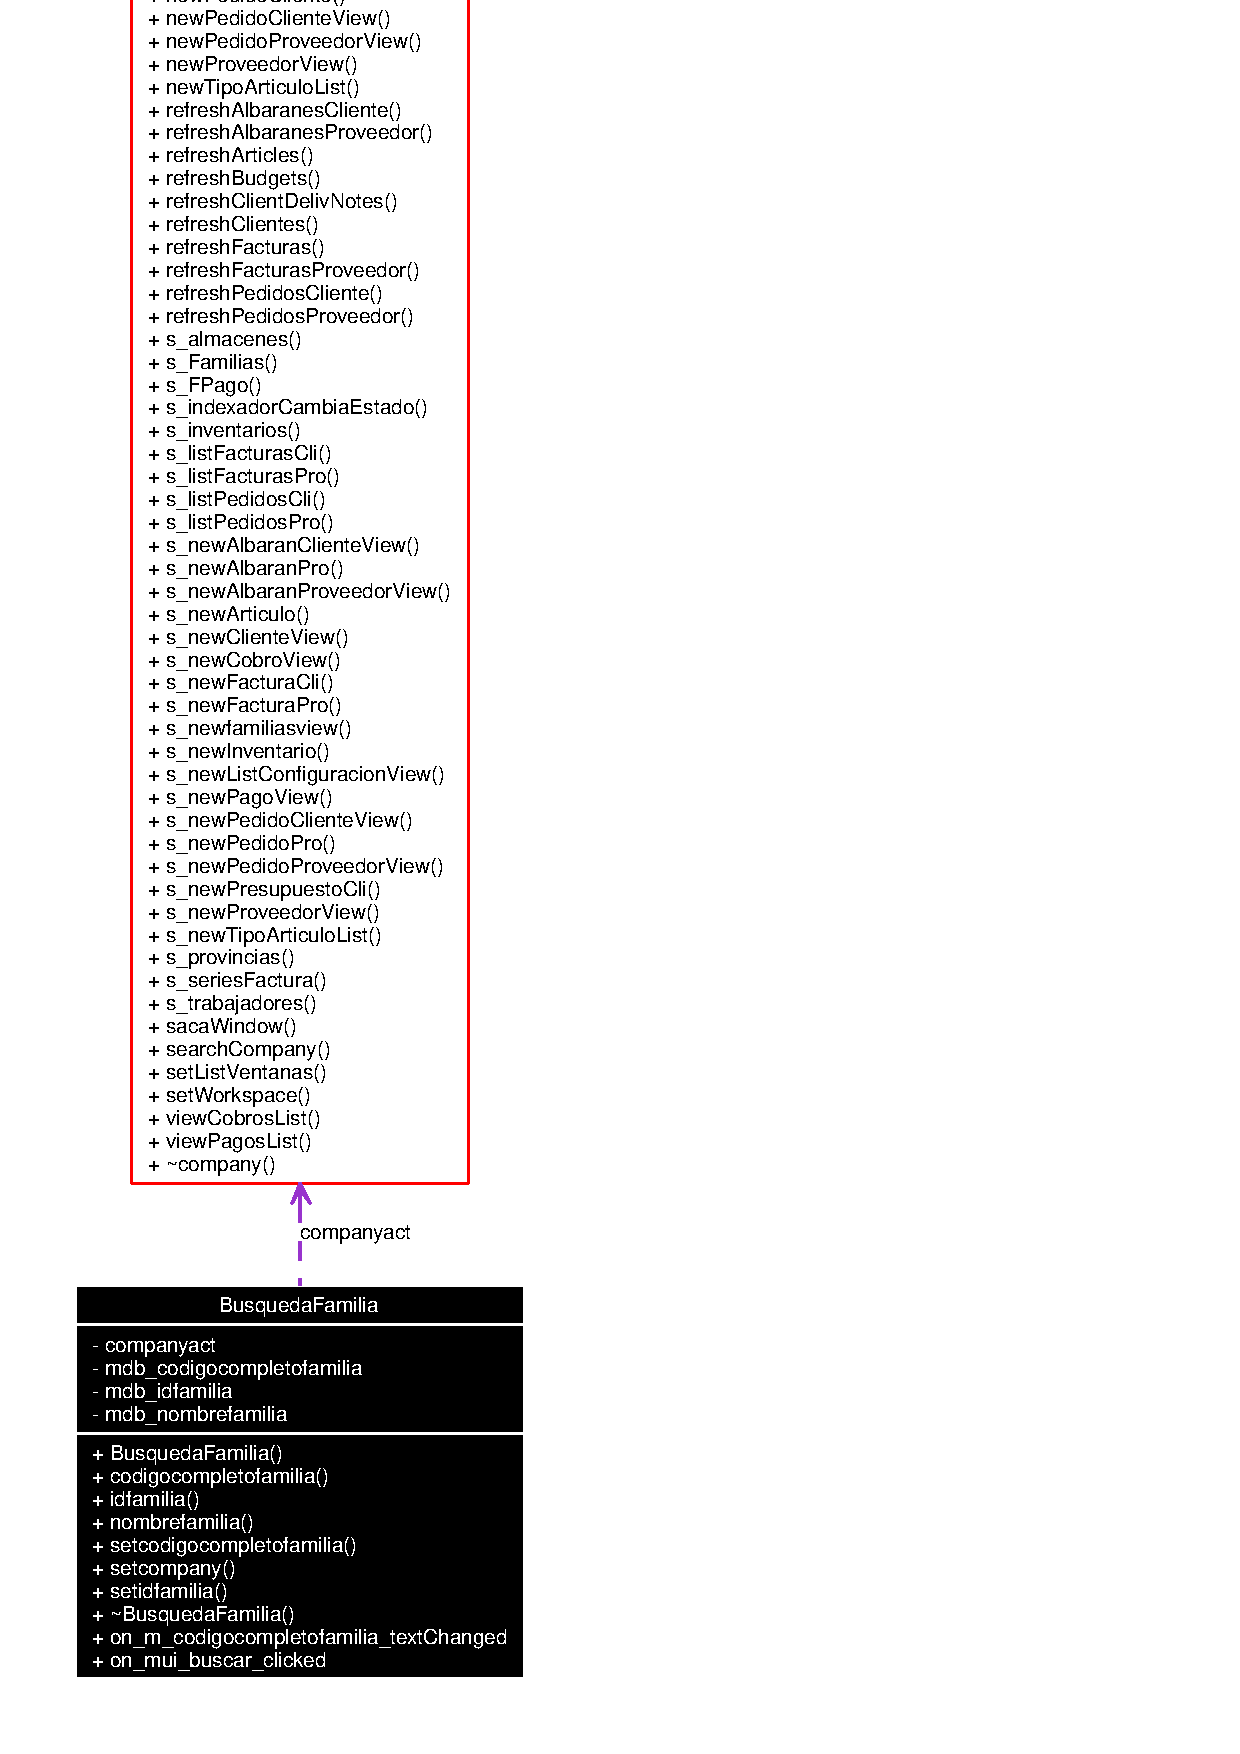
\includegraphics[width=126pt]{classBusquedaFamilia__coll__graph}
\end{center}
\end{figure}
\subsection*{Slots p\'{u}blicos}
\begin{CompactItemize}
\item 
virtual void {\bf on\_\-m\_\-codigocompletofamilia\_\-text\-Changed} (const QString \&)\label{classBusquedaFamilia_i0}

\item 
virtual void {\bf on\_\-mui\_\-buscar\_\-clicked} ()\label{classBusquedaFamilia_i1}

\begin{CompactList}\small\item\em Busqueda de familias. \item\end{CompactList}\end{CompactItemize}
\subsection*{Se\~{n}ales}
\begin{CompactItemize}
\item 
void {\bf value\-Changed} (QString)\label{classBusquedaFamilia_l0}

\end{CompactItemize}
\subsection*{M\'{e}todos p\'{u}blicos}
\begin{CompactItemize}
\item 
{\bf Busqueda\-Familia} (QWidget $\ast$parent=0)\label{classBusquedaFamilia_a0}

\item 
virtual QString {\bf codigocompletofamilia} ()\label{classBusquedaFamilia_a1}

\item 
virtual QString {\bf idfamilia} ()\label{classBusquedaFamilia_a2}

\item 
virtual QString {\bf nombrefamilia} ()\label{classBusquedaFamilia_a3}

\item 
virtual void {\bf setcodigocompletofamilia} (QString val)\label{classBusquedaFamilia_a4}

\item 
void {\bf setcompany} ({\bf company} $\ast$comp)\label{classBusquedaFamilia_a5}

\item 
virtual void {\bf setidfamilia} (QString val)\label{classBusquedaFamilia_a6}

\end{CompactItemize}


\subsection{Descripci\'{o}n detallada}
Permite buscar y seleccionar una familia de art\'{\i}culos. 

Muestra la parte del formulario que permite buscar y seleccionar una familia de art\'{\i}culos. 



La documentaci\'{o}n para esta clase fu\'{e} generada a partir de los siguientes archivos:\begin{CompactItemize}
\item 
busquedafamilia.h\item 
busquedafamilia.cpp\end{CompactItemize}
